\documentclass[aspectratio=169]{beamer}
\usepackage{amsmath}
\usepackage{amssymb}
\usepackage{minted}
\usepackage{graphicx}
\title{Stochastic Gradient Descent}
\subtitle{Log-logistic  dose-response curve}
\author{Lucas Støjko Andersen}
\setminted{fontsize=\fontsize{8pt}{8pt}}
\institute{University of Copenhagen}
\date{\today}

\begin{document}
\begin{frame}
    \titlepage
\end{frame}
\begin{frame}
    \frametitle{Stochastic Gradient Descent}
    \framesubtitle{Online learning}
    Assume $L(X,\theta)$ is a loss function we then minimize the expected loss
    \begin{equation}
        H(\theta)=E(L(X,\theta)).
    \end{equation}
    If differentiation and expectation can interchange then
    \begin{equation}
        \nabla H(\theta)=E(\nabla L(X,\theta))
    \end{equation}
    and if $X_{1},X_{2},\ldots$ are i.i.d. then $\nabla L(X_{i},\theta)$ is an unbiased estimator of $E(\nabla L(X,\theta))$. We then perform gradient descent using sampled $L(X_{i},\theta)$:
    \begin{equation}
        \theta_{n+1}=\theta_{n} - \gamma_{n}\nabla L(X_{n+1},\theta_{n}).
    \end{equation}
    where $\gamma_{n}>0$ is a learning rate.
\end{frame}
\begin{frame}
    \frametitle{Stochastic Gradient Descent}
    \framesubtitle{Batch learning}
    We replace $H$ with
    \begin{equation}
        H_{N}(\theta)=\frac{1}{N}\sum_{i=1}^{N}L(X_{i},\theta)
    \end{equation}
    and minimize $H_{N}$ instead. We sample from the empirical distribution of the observations and use the online learning approach.
\end{frame}
\begin{frame}[fragile]
    \frametitle{Implementation of Stochastic Gradient Descent}
\begin{minted}[fontsize=\fontsize{7pt}{7pt}]{r}
SGD_1 <- function(par0,
                  loss_gr,
                  N,
                  gamma0 = 1,
                  maxit = 15,
                  loss = NULL,
                  cb = NULL) {
  if(is.numeric(gamma0)) {
    if(length(gamma0) == 1) {
      gamma <- rep(gamma0, maxit)
    } else {
      gamma <- c(gamma0, rep(gamma0[length(gamma0)], maxit - length(gamma0)))
    }
  } else if (is.function(gamma0)) {
    gamma <- gamma0(1:maxit)
  } else {
    stop("gamma0 must be a numeric or a function.")
  }
  par <- par0
  for(i in 1:maxit) {
    index <- sample(N)
    for(j in 1:N) {
      gr <- loss_gr(par, index[j])
      par <- par - gamma[i] * gr
    }
    if(!is.null(cb)) cb()
    par0 <- par
  }
  par
}
\end{minted}
\end{frame}
\begin{frame}
    \frametitle{Log-logistic dose-response curve}
    For $\alpha,\beta,\gamma,\rho\in\mathbb{R}$ consider
    \begin{equation}
        f(x\mid\alpha,\beta,\gamma,\rho)=\gamma + \frac{\rho - \gamma}{1 + e^{\beta\log(x)-\alpha}}.
    \end{equation}
    Let $Y_{i}=f(X_{i}\mid\alpha,\beta,\gamma,\rho)+\varepsilon_{i}$ with $\varepsilon_{i}\sim\mathcal{N}(0,\sigma^{2})$ independent.\\[12pt]
    We generate $\log X_{i}$ from $\mathcal{N}(0,\omega^{2})$ and generate $Y_{i}$ by the above. We aim to minimize the empirical loss
    \begin{equation}
        \frac{1}{N}\sum_{i=1}^{N}(Y_{i}-f(X_{i}\mid\alpha,\beta,\gamma,\rho))^{2}.
    \end{equation}
\end{frame}
\begin{frame}
    \frametitle{Log-logistc dose-response curve}
    \framesubtitle{Plot of generated data}
    With $\omega = 2$, $\sigma = 0.5$, $\alpha = 2$, $\beta = 3$, $\gamma = 5$ and $\rho = 1$ we plot the generated data for 1.000 observations.
    \begin{figure}
        \centering
        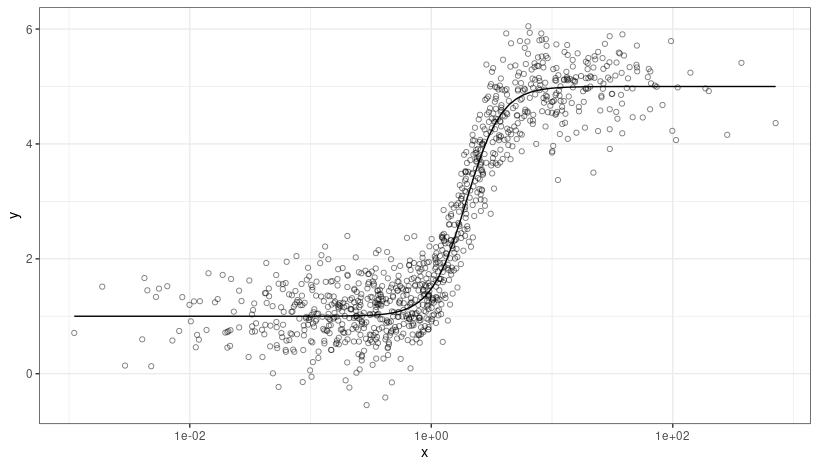
\includegraphics[scale = 0.4]{figure/dataplot.png}
    \end{figure}
\end{frame}
\begin{frame}[fragile]
    \frametitle{Result of Stochastic Gradient Descent}
\begin{minted}{r}
opt_value <- optim(c(2, 3, 5, 1), log_loss(X, Y))$value
SGD_tracer <- tracer("par")
SGD_1(c(-1, 6, 3, 3), 
        log_gradient(X, Y),
        N = length(X),
        gamma0 = decay_scheduler(gamma0 = 0.5, gamma1 = 0.01, n1 = 200),
        maxit = 200,
        loss = log_loss(X, Y),
        cb = SGD_tracer$tracer)
\end{minted}
    \begin{align*}
        &\theta_{\text{SGD}}=(1.815715, 2.797085, 5.006571, 0.959967) \\
        &\theta_{\text{optim}}=(1.820240, 2.789082, 5.001176, 0.965572)
    \end{align*}
\end{frame}
\begin{frame}
    \frametitle{Result of Stochastic Gradient Descent}
    \framesubtitle{Plot of loss value of optim vs SGD}
    \begin{figure}
        \centering
        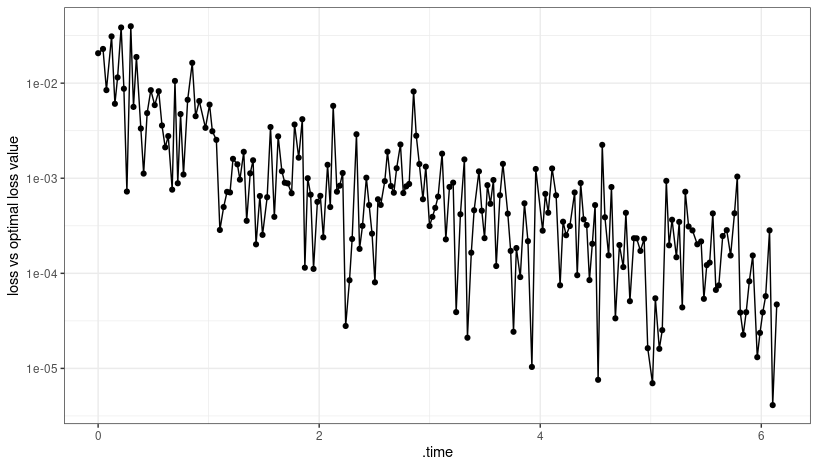
\includegraphics[scale = 0.4]{figure/SGD1_loss.png}
    \end{figure}
\end{frame}
\begin{frame}[fragile]
    \frametitle{Abstracting the Implementation of SGD}
\begin{minted}{r}
SGD <- function(par0,
                loss_gr,
                N,
                batch,
                epoch,
                gamma0 = 1,
                maxit = 15,
                loss,
                cb = NULL) {
  if(is.numeric(gamma0)) {
    if(length(gamma0) == 1) {
      gamma <- rep(gamma0, maxit)
    } else {
      gamma <- c(gamma0, rep(gamma0[length(gamma0)], maxit - length(gamma0)))
    }
  } else if (is.function(gamma0)) {
    gamma <- gamma0(1:maxit)
  } else {
    stop("gamma0 must be a numeric or a function.")
  }
  for(i in 1:maxit) {
    index <- batch(N)
    par <- epoch(par0, index, loss_gr, gamma[i])
    if(!is.null(cb)) cb()
    par0 <- par
  }
  par
}
\end{minted}
\end{frame}
\begin{frame}[fragile]
    \frametitle{Batch Implementation}
\begin{minted}{r}
batch_random <- function(batch_size = NULL, replace = FALSE) {
  if(!is.null(batch_size)) batch_size <- as.integer(batch_size)
  function(N) {
    if(is.null(batch_size)) batch_size <<- N
    if(batch_size <= N) return(sample(N, batch_size, replace = replace))
    sample(N, batch_size, replace = TRUE)
  }
}
\end{minted}
\end{frame}
\begin{frame}[fragile]
    \frametitle{Another Batch Implementation}
\begin{minted}[fontsize=\fontsize{7pt}{7pt}]{r}
batch_random_chunk <- function(size, 
                               chunks = 1L, 
                               replace = FALSE, 
                               shuffle = FALSE) {
  shuffle_index <- NULL
  force(shuffle)
  function(N) {
    if(shuffle & is.null(shuffle_index)) rand_indicies <- sample(N)
    max_chunk <- max(1, floor(N / size) - 1)
    if(is.infinite(chunks)) chunks <- max_chunk
    if(chunks <= max_chunk) {
      chunk_id <- sample(1:max_chunk, replace = replace)
    } else {
      chunk_id <- sample(1:max_chunk, chunks, replace = TRUE)
    }
    index <- numeric(chunks * size)
    if(is.null(shuffle_index)) {
        for(i in seq_along(chunk_id)) {
          index[((i - 1) * size + 1):(i * size)] <-
          ((chunk_id[i] - 1) * size + 1):(chunk_id[i] * size)
        }
    } else {
        for(i in seq_along(chunk_id)) {
          index[((i - 1) * size + 1):(i * size)] <-
            shuffle_index[((chunk_id[i] - 1) * size + 1):(chunk_id[i] * size)]
        }
    }
    index
  }
}
\end{minted}
\end{frame}
\begin{frame}[fragile]
    \frametitle{Epoch Implementation}
\begin{minted}[]{r}
epoch_batch <- function(mini_batch_size = 1) {
  function(par0, index, loss_gr, gamma) {
    mini_batch_size <- min(length(index), mini_batch_size)
    M <- floor(length(index) / mini_batch_size)
    par <- par0
    for(i in 1:M) {
      mini_batch_index <- ((i - 1) * mini_batch_size + 1):(i * mini_batch_size)
      gr <- loss_gr(par, index[mini_batch_index])
      par <- par - gamma * gr
    }
    par
  }
}

epoch_full <- function() {
  function(par0, index, loss_gr, gamma) {
    for(i in 1:length(index)) {
      gr <- loss_gr(par0, index[i])
      par0 <- par0 - gamma * gr
    }
    par0
  }
}
\end{minted}
\end{frame}
\begin{frame}[fragile]
    \frametitle{Testing Against the First Implementation}
\begin{minted}{r}
SGD_tracer2 <- tracer("par")
SGD(par0 = c(-1, 6, 3, 3),
    loss_gr = log_gradient(X, Y),
    N = length(X),
    batch = batch_random(),
    epoch = epoch_full(),
    gamma0 = decay_scheduler(gamma0 = 1, gamma1 = 0.2, n1 = 200),
    loss = log_loss(X, Y),
    maxit = 200,
    cb = SGD_tracer2$tracer)
\end{minted}
The abstract implementation yields
\begin{equation}
    \theta_{\text{SGD}}=(1.8175899, 2.7902753, 4.9934073, 0.9892618).
\end{equation}
\end{frame}
\begin{frame}
    \frametitle{Testing Against the First Implementation}
    \begin{figure}
        \centering
        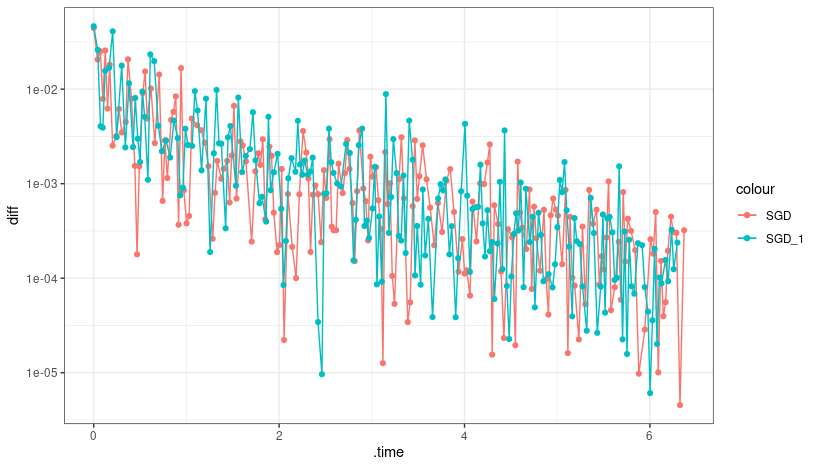
\includegraphics[scale = 0.4]{figure/ComparisonSGD_1.png}
    \end{figure}
\end{frame}
\begin{frame}[fragile]
    \frametitle{Mini Batch vs Batch}
\begin{minted}{r}
SGD_tracer3 <- tracer("par")
SGD(par0 = c(-1, 6, 3, 3),
    loss_gr = log_gradient(X, Y),
    N = length(X),
    batch = batch_random(),
    epoch = epoch_batch(100),
    gamma0 = decay_scheduler(gamma0 = 1, gamma1 = 0.1, n1 = 1000),
    maxit = 1000,
    loss = log_loss(X, Y),
    cb = SGD_tracer3$tracer)
\end{minted}
\end{frame}
\begin{frame}
    \frametitle{Mini Batch vs Batch}    
    \begin{figure}
        \centering
        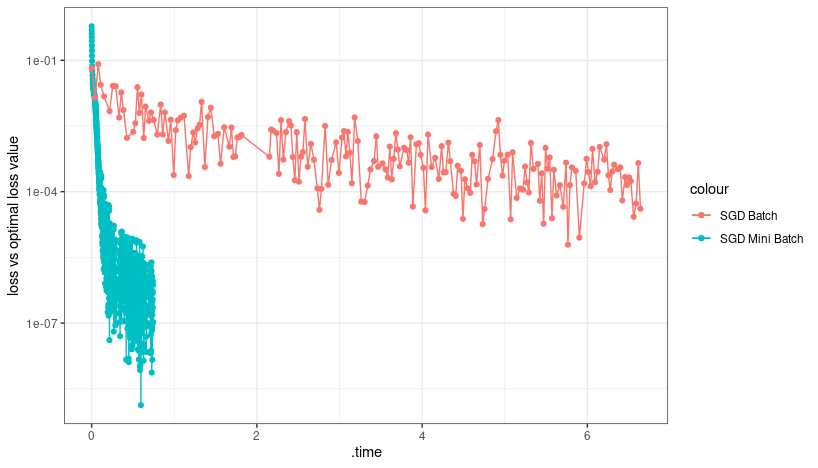
\includegraphics[scale = 0.6]{figure/BatchVsMini.png}
    \end{figure}
\end{frame}
\begin{frame}[fragile]
    \frametitle{Comparison to Gradient Descent Algorithm}    
\begin{minted}[fontsize=\fontsize{6.5pt}{6.5pt}]{r}
GD <- function(par0, 
               loss, 
               loss_gr, 
               d = 0.8, 
               c = 0.1, 
               gamma0 = 1,
               maxit = 500,
               stop_criteria = NULL,
               backtrack = TRUE,
               cb = NULL) {
  for(i in 1:maxit) {
    if(backtrack) value <- loss(par0)
    grad <- loss_gr(par0)
    h_prime <- sum(grad^2)
    gamma <- gamma0
    par <- par0 - gamma * grad
    if(backtrack) {
      while(loss(par) > value - c * gamma * h_prime) {
        gamma <- d * gamma
        par <- par0 - gamma * grad
      }
    }
    if(!is.null(cb)) cb()
    if(!is.null(stop_criteria)) {
      if(stop_criteria(par, par0, loss_gr, loss)) break
    }
    par0 <- par
  }
  if(i == maxit)
    warning("Maximal number, ", maxit, ", of iterations reached")
  par
}
\end{minted}
\end{frame}
\begin{frame}[fragile]
    \frametitle{Stopping criteria}
\begin{minted}{r}
stop_parm <- function(epsilon, k) {
  force(epsilon)
  force(k)
  n <- 0
  function(par0, par, loss_gr, loss) {
    if(norm(par0 - par, "2") < 
       epsilon * (norm(par0, "2") + epsilon)) {
      n <<- n + 1
    } else {
      n <<- 0
    }
    n == k
  }
}
\end{minted}
\end{frame}
\begin{frame}[fragile]
    \frametitle{SGD vs. GD}  
\begin{minted}{r}
GD_tracer <- tracer("par", N = 0)
GD(par0 = c(-1, 6, 3, 3),
   loss = log_loss(X, Y),
   loss_gr = log_gradient(X, Y),
   gamma0 = 1,
   maxit = 100000,
   stop_criteria = stop_parm(1e-5, 3),
   backtrack = FALSE,
   cb = GD_tracer$tracer)
\end{minted}
\end{frame}
\begin{frame}[fragile]
    \frametitle{SGD vs. GD}
\begin{minted}{r}
SGD_tracer4 <- tracer("par", N = 0)
SGD(par0 = c(-1, 6, 3, 3),
    loss_gr = log_gradient(X, Y),
    N = length(X),
    batch = batch_random(),
    epoch = epoch_batch(200),
    gamma0 = decay_scheduler(gamma0 = 1, gamma1 = 0.05, a = 2, n1 = 1000),
    maxit = 100000,
    stop_criteria = stop_parm(1e-5, 3),
    cb = SGD_tracer4$tracer)

SGD_tracer5 <- tracer("par", N = 0)
SGD(par0 = c(-1, 6, 3, 3),
    loss_gr = log_gradient(X, Y),
    N = length(X),
    batch = batch_random(),
    epoch = epoch_batch(200),
    gamma0 = 0.1,
    maxit = 100000,
    stop_criteria = stop_parm(1e-5, 3),
    cb = SGD_tracer5$tracer)
\end{minted}
\end{frame}
\begin{frame}
    \frametitle{SGD vs. GD}
    \begin{figure}
        \centering
        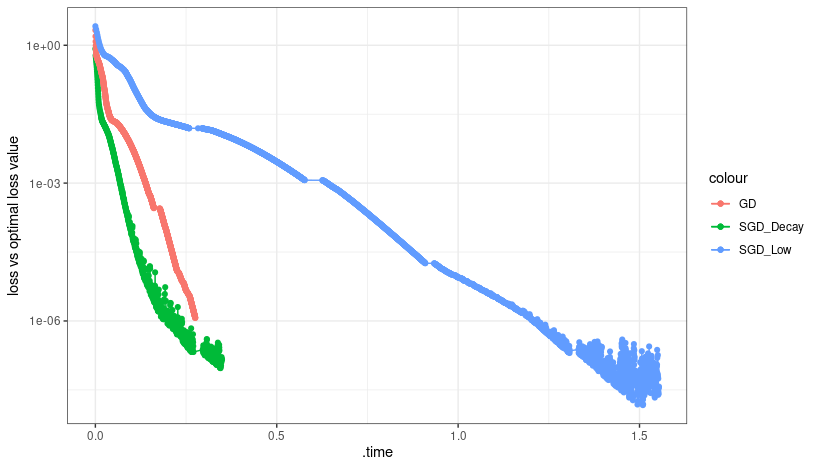
\includegraphics[scale = 0.4]{figure/GD_Comparison.png}
    \end{figure}
\end{frame}
\begin{frame}[fragile]
    \frametitle{SGD vs. GD}
    \framesubtitle{Large Sample Size}
    Generate 100.000 samples.
\begin{minted}{r}
GD_tracer2 <- tracer("par", N = 0)
GD(par0 = c(-1, 6, 3, 3),
   loss = log_loss(X_big, Y_big),
   loss_gr = log_gradient(X_big, Y_big),
   gamma0 = 1,
   maxit = 10000,
   stop_criteria = stop_parm(1e-5, 3),
   backtrack = FALSE,
   cb = GD_tracer2$tracer)

SGD_tracer5 <- tracer("par", N = 0)
SGD(par0 = c(-1, 6, 3, 3),
    loss_gr = log_gradient(X_big, Y_big),
    N = length(X_big),
    batch = batch_random(10000, replace = TRUE),
    epoch = epoch_batch(1000),
    gamma0 = decay_scheduler(gamma0 = 1, gamma1 = 0.01, a = 2, n1 = 1000),
    stop_criteria = stop_parm(1e-5, 3),
    maxit = 10000,
    cb = SGD_tracer5$tracer)
\end{minted}
\end{frame}
\begin{frame}
    \frametitle{SGD vs. GD}
    \framesubtitle{Large Sample Size}
    \begin{figure}
        \centering
        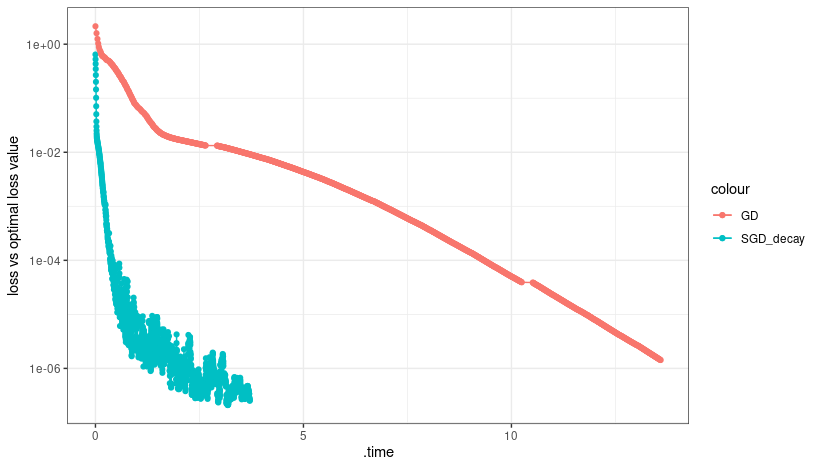
\includegraphics[scale = 0.5]{figure/100kComp.png}
    \end{figure}
\end{frame}
\begin{frame}
    \frametitle{Profiling SGD Implementation Using \texttt{profvis} Package}
    \begin{figure}
        \centering
        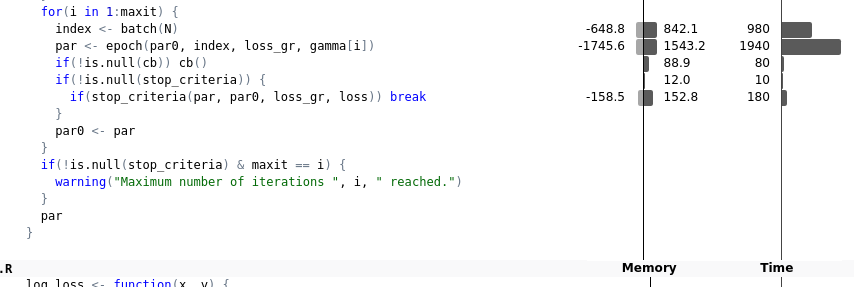
\includegraphics[scale = 0.4]{figure/SGDProf.png}
    \end{figure}
\end{frame}
\begin{frame}
    \frametitle{Profiling SGD Implementation Using \texttt{profvis} Package}
    \begin{figure}
        \centering
        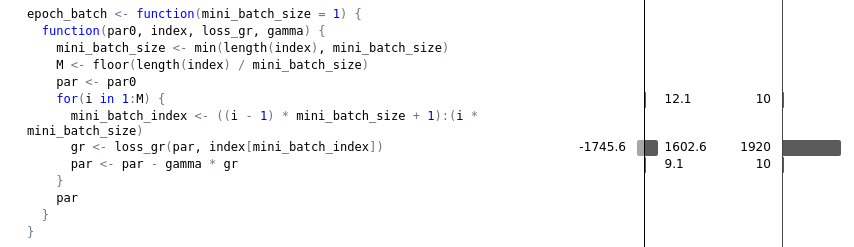
\includegraphics[scale = 0.4]{figure/EpochProf.png}
    \end{figure}
\end{frame}
\begin{frame}[fragile]
    \frametitle{Implementation of Gradient Using \texttt{Rcpp}}
\begin{minted}{cpp}
#include <Rcpp.h>

using namespace Rcpp;

// [[Rcpp::export]]
NumericVector gradient_rcpp(NumericVector par,
                            NumericVector x,
                            NumericVector y) {
  int N = x.size();
  NumericVector gr(4);
  for(int i = 0; i < N; ++i) {
    double elogx, da, db, dg, dr, yf, logx;
    logx = std::log(x[i]);
    elogx = std::exp(par[1] * logx - par[0]);
    dr = 1 / (1 + elogx);
    dg = 1 - dr;
    da = elogx * (par[3] - par[2]) * dr * dr;
    db = -da * logx;
    yf = y[i] - par[2] - (par[3] - par[2]) * dr;
    gr[0] -= da * yf / 2;
    gr[1] -= db * yf / 2;
    gr[2] -= dg * yf / 2;
    gr[3] -= dr * yf / 2;
  }
  return gr / N;
}   
\end{minted}
\end{frame}
\begin{frame}[fragile]
    \frametitle{Implementation of Mini Batch Epoch Using \texttt{Rcpp} Package}
\begin{minted}{cpp}
// [[Rcpp::export]]
NumericVector epoch_rcpp(NumericVector par0, 
                    NumericVector x, 
                    NumericVector y,
                    int minisize,
                    double gamma) {
  int n, MAX;
  Range r(0, minisize - 1);
  
  n = x.size();
  MAX = std::floor(n / minisize);
  NumericVector par = clone(par0);
  
  for(int i = 0; i < MAX; ++i, r += minisize) {
     par = par - gamma * gradient_rcpp(par, x[r], y[r]);
  }

  return par;
}
\end{minted}
\end{frame}
\begin{frame}[fragile]
    \frametitle{Implementation of Mini Batch Epoch Using \texttt{Rcpp} Package}
    \framesubtitle{Calling Gradient from R}
\begin{minted}{cpp}
// [[Rcpp::export]]
NumericVector epoch_rcpp_partial(NumericVector par0,
                                 NumericVector index,
                                 Function gr,
                                 int minisize,
                                 double gamma) {
  
  int n = index.size();
  int MAX = std::floor(n / minisize);
  NumericVector par = clone(par0);
  
  Range r(0, minisize - 1);
  
  for(int i = 0; i < MAX; ++i, r += minisize) {
    NumericVector gr_tmp = gr(par, index[r]);
    par = par - gamma * gr_tmp;
  }
  
  return par;
}
\end{minted}
\end{frame}
\begin{frame}
    \frametitle{Benchmark Using \texttt{bench} Package}
    \begin{figure}
        \centering
        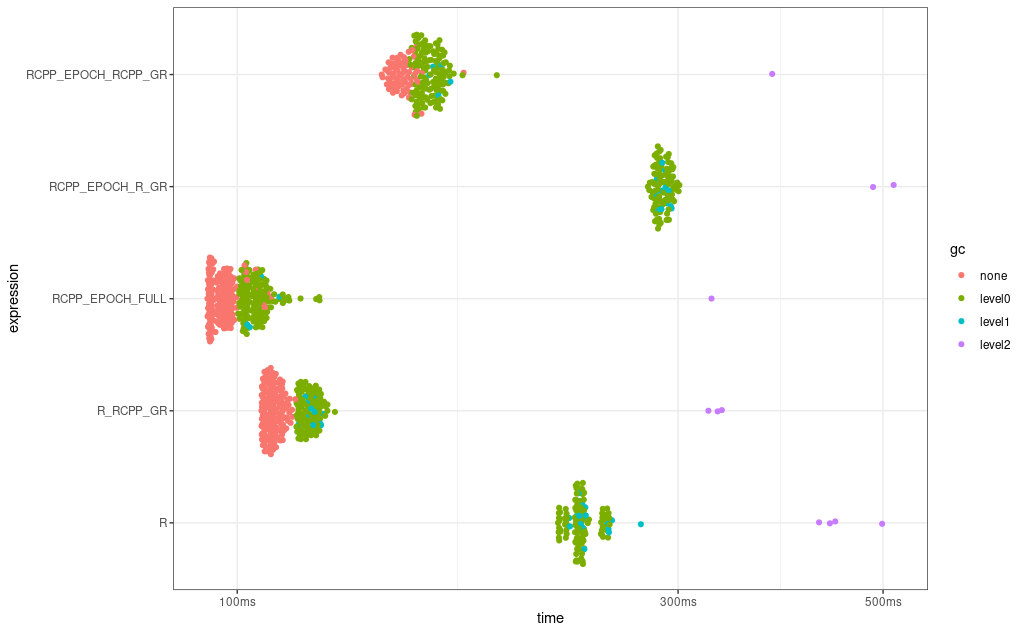
\includegraphics[scale = 0.4]{figure/RcppVR.png}
    \end{figure}
\end{frame}
\begin{frame}[fragile]
    \frametitle{Epoch Implementation Using R's C API}
\begin{minted}[fontsize = \fontsize{7pt}{7pt}]{c}
SEXP epoch_batch(SEXP par0, SEXP index, SEXP loss_gr, SEXP gamma, SEXP mbs, SEXP rho) {
  int mbs2, M, n;
  n = length(par0);
  if(INTEGER(mbs)[0] > length(index)) {
    mbs2 = length(index);
  } else {
    mbs2 = INTEGER(mbs)[0];
  }
  M = floor(length(index) / mbs2);
  SEXP gr_call = PROTECT(lang3(loss_gr, R_NilValue, R_NilValue));
  SEXP par = PROTECT(allocVector(REALSXP, n));
  SEXP m_index = PROTECT(allocVector(INTSXP, mbs2));
  int *iptr = INTEGER(index);
  int *miptr = INTEGER(m_index);
  for(int i = 0; i < n; ++i)
    REAL(par)[i] = REAL(par0)[i];
  for(int i = 0; i < M; ++i) {
    for(int j = 0; j < mbs2; ++j)
      miptr[j] = iptr[i * mbs2 + j];
    SETCADR(gr_call, par);
    SETCADDR(gr_call, m_index);
    SEXP gr = eval(gr_call, rho);
    for(int k = 0; k < n; ++k)
      REAL(par)[k] = REAL(par)[k] - REAL(gamma)[0] * REAL(gr)[k];
  }
  UNPROTECT(3);
  return par;
}
\end{minted}
\end{frame}
\begin{frame}[fragile]
    \frametitle{SGD Implementation Using R's C API}
\begin{minted}[fontsize = \fontsize{7pt}{7pt}]{c}
#include <Rinternals.h>
#include <R.h>

SEXP sgd(SEXP par0, SEXP loss_gr, SEXP N, SEXP batch, SEXP epoch, SEXP gamma0, SEXP maxit, SEXP rho) {
  int n_maxit = asInteger(maxit);
  double *gam = REAL(gamma0);
  SEXP par = PROTECT(allocVector(REALSXP, length(par0)));
  for(int i = 0; i < length(par0); ++i)
    REAL(par)[i] = REAL(par0)[i];
  SEXP batch_call = PROTECT(lang2(batch, R_NilValue));
  SEXP s, t;
  for(int i = 0; i < n_maxit; ++i) {
    SETCADR(batch_call, N);
    SEXP index = eval(batch_call, rho);
    SEXP gami = PROTECT(ScalarReal(gam[i]));
    t = s = PROTECT(allocList(5));
    SET_TYPEOF(s, LANGSXP);
    SETCAR(t, epoch); t = CDR(t);
    SETCAR(t, par); t = CDR(t);
    SETCAR(t, index); t = CDR(t);
    SETCAR(t, loss_gr); t = CDR(t);
    SETCAR(t, gami);
    par = eval(s, rho);
    UNPROTECT(2);
  }
  UNPROTECT(2);
  return par;
}
\end{minted}
\end{frame}
\begin{frame}[fragile]
    \frametitle{SGD Implementation Using R's C API}
    Build shared library using \texttt{R CMD SHLIB} command.\\[12pt]
\begin{minted}{r}
dyn.load("c/src/sgd_o.o")

epoch_test <- function(mini_batch_size = 1L) {
  function(par0, index, loss_gr, gamma0) {
    .Call("epoch_batch",
          par0,
          index,
          loss_gr,
          gamma0,
          mini_batch_size,
          environment())
  }
}
\end{minted}
\end{frame}
\begin{frame}
    \frametitle{SGD Implementation Benchmark}
    \begin{figure}
        \centering
        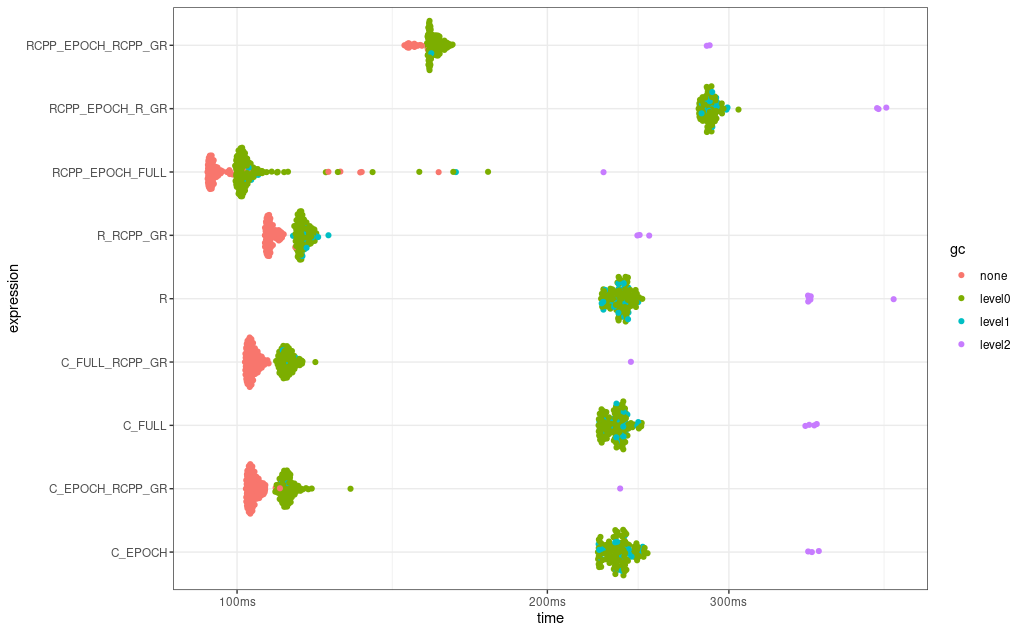
\includegraphics[scale = 0.4]{figure/RcppVcVr.png}
    \end{figure}
\end{frame}
\begin{frame}
    \frametitle{SGD Implementation Benchmark}
    \begin{figure}
        \centering
        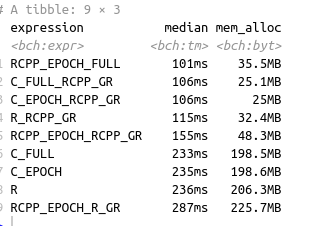
\includegraphics[scale = 0.6]{figure/table.png}
    \end{figure}
\end{frame}
\end{document}
